%% LyX 2.4.0~beta5 created this file.  For more info, see https://www.lyx.org/.
%% Do not edit unless you really know what you are doing.
\documentclass[french,english,footrule]{foils}
\usepackage[T1]{fontenc}
\usepackage[latin9]{inputenc}
\usepackage{geometry}
\geometry{verbose}
\setcounter{secnumdepth}{1}
\setcounter{tocdepth}{1}
\synctex=-1
\usepackage{xcolor}
\usepackage{babel}
\usepackage{fancybox}
\usepackage{calc}
\usepackage{url}
\usepackage{amsmath}
\usepackage{amsthm}
\usepackage{amssymb}
\usepackage{graphicx}
\usepackage[pdfusetitle,
 bookmarks=true,bookmarksnumbered=false,bookmarksopen=false,
 breaklinks=false,pdfborder={0 0 1},backref=false,colorlinks=false]
 {hyperref}

\makeatletter

%%%%%%%%%%%%%%%%%%%%%%%%%%%%%% LyX specific LaTeX commands.
\newcommand{\noun}[1]{\textsc{#1}}

%%%%%%%%%%%%%%%%%%%%%%%%%%%%%% Textclass specific LaTeX commands.
\theoremstyle{definition}
\newtheorem{defn}{\protect\definitionname}

%%%%%%%%%%%%%%%%%%%%%%%%%%%%%% User specified LaTeX commands.
\usepackage{graphicx,xcolor}
% darker colors for better slides...
\definecolor{green}{RGB}{0, 180, 0}
\definecolor{cyan}{RGB}{0, 180, 180}
\definecolor{yellow}{RGB}{211,211,0}

%\usepackage{xcolor}
\renewcommand{\labelitemi}{$\textcolor{blue}{\bullet}$}
\renewcommand{\labelitemii}{$\textcolor{teal}{\Rightarrow}$}
\renewcommand{\labelitemiii}{$\textcolor{red}{\rightarrow}$}
\renewcommand{\labelitemiv}{$\textcolor{brown}{\circ}$}

\newcommand{\T}{\mathrm{T}}  % transpose
\newcommand{\PP}{\mathrm{P}}  % probability
\newcommand{\dd}{\mathrm{d}} % integration dx
\newcommand{\ee}{\mathrm{e}} % exponential
\newcommand{\E}{\mathrm{E}} % expectation

\makeatother

\addto\captionsenglish{\renewcommand{\definitionname}{Definition}}
\addto\captionsfrench{\renewcommand{\definitionname}{D�finition}}
\providecommand{\definitionname}{Definition}

\begin{document}
\title{DA - Adjoint Method\\
\rule[0.5ex]{1\columnwidth}{3pt}}
\author{Mark Asch - CSU/IMU/2023}
\date{\bigskip{}
\bigskip{}
\bigskip{}
\noun{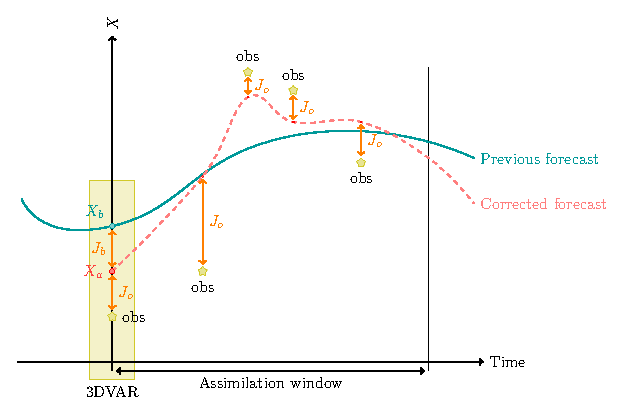
\includegraphics[scale=1.2]{graphics/3D4D-Var}}}
\maketitle

\MyLogo{Data Assim. - Adjoints - M. Asch - Lecture 02}

\foilhead{Outline of the course (I)}

\textcolor{blue}{Adjoint methods and variational data assimilation
(4h)}
\begin{enumerate}
\item Introduction to data assimilation: setting, history, overview, definitions.
\item \textcolor{red}{Adjoint method.}
\item \textcolor{lightgray}{Variational data assimilation methods: }
\begin{enumerate}
\item \textcolor{lightgray}{3D-Var, }
\item \textcolor{lightgray}{4D-Var.}
\end{enumerate}
\end{enumerate}

\foilhead{Outline of the course (II)}

\textcolor{blue}{Statistical estimation, Kalman filters and sequential
data assimilation (4h)}
\begin{enumerate}
\item \textcolor{lightgray}{Introduction to statistical DA.
\item Statistical estimation.
\item The Kalman filter.
\item Nonlinear extensions and ensemble filters.}
\end{enumerate}

\foilhead{Reference Textbooks}
\begin{center}
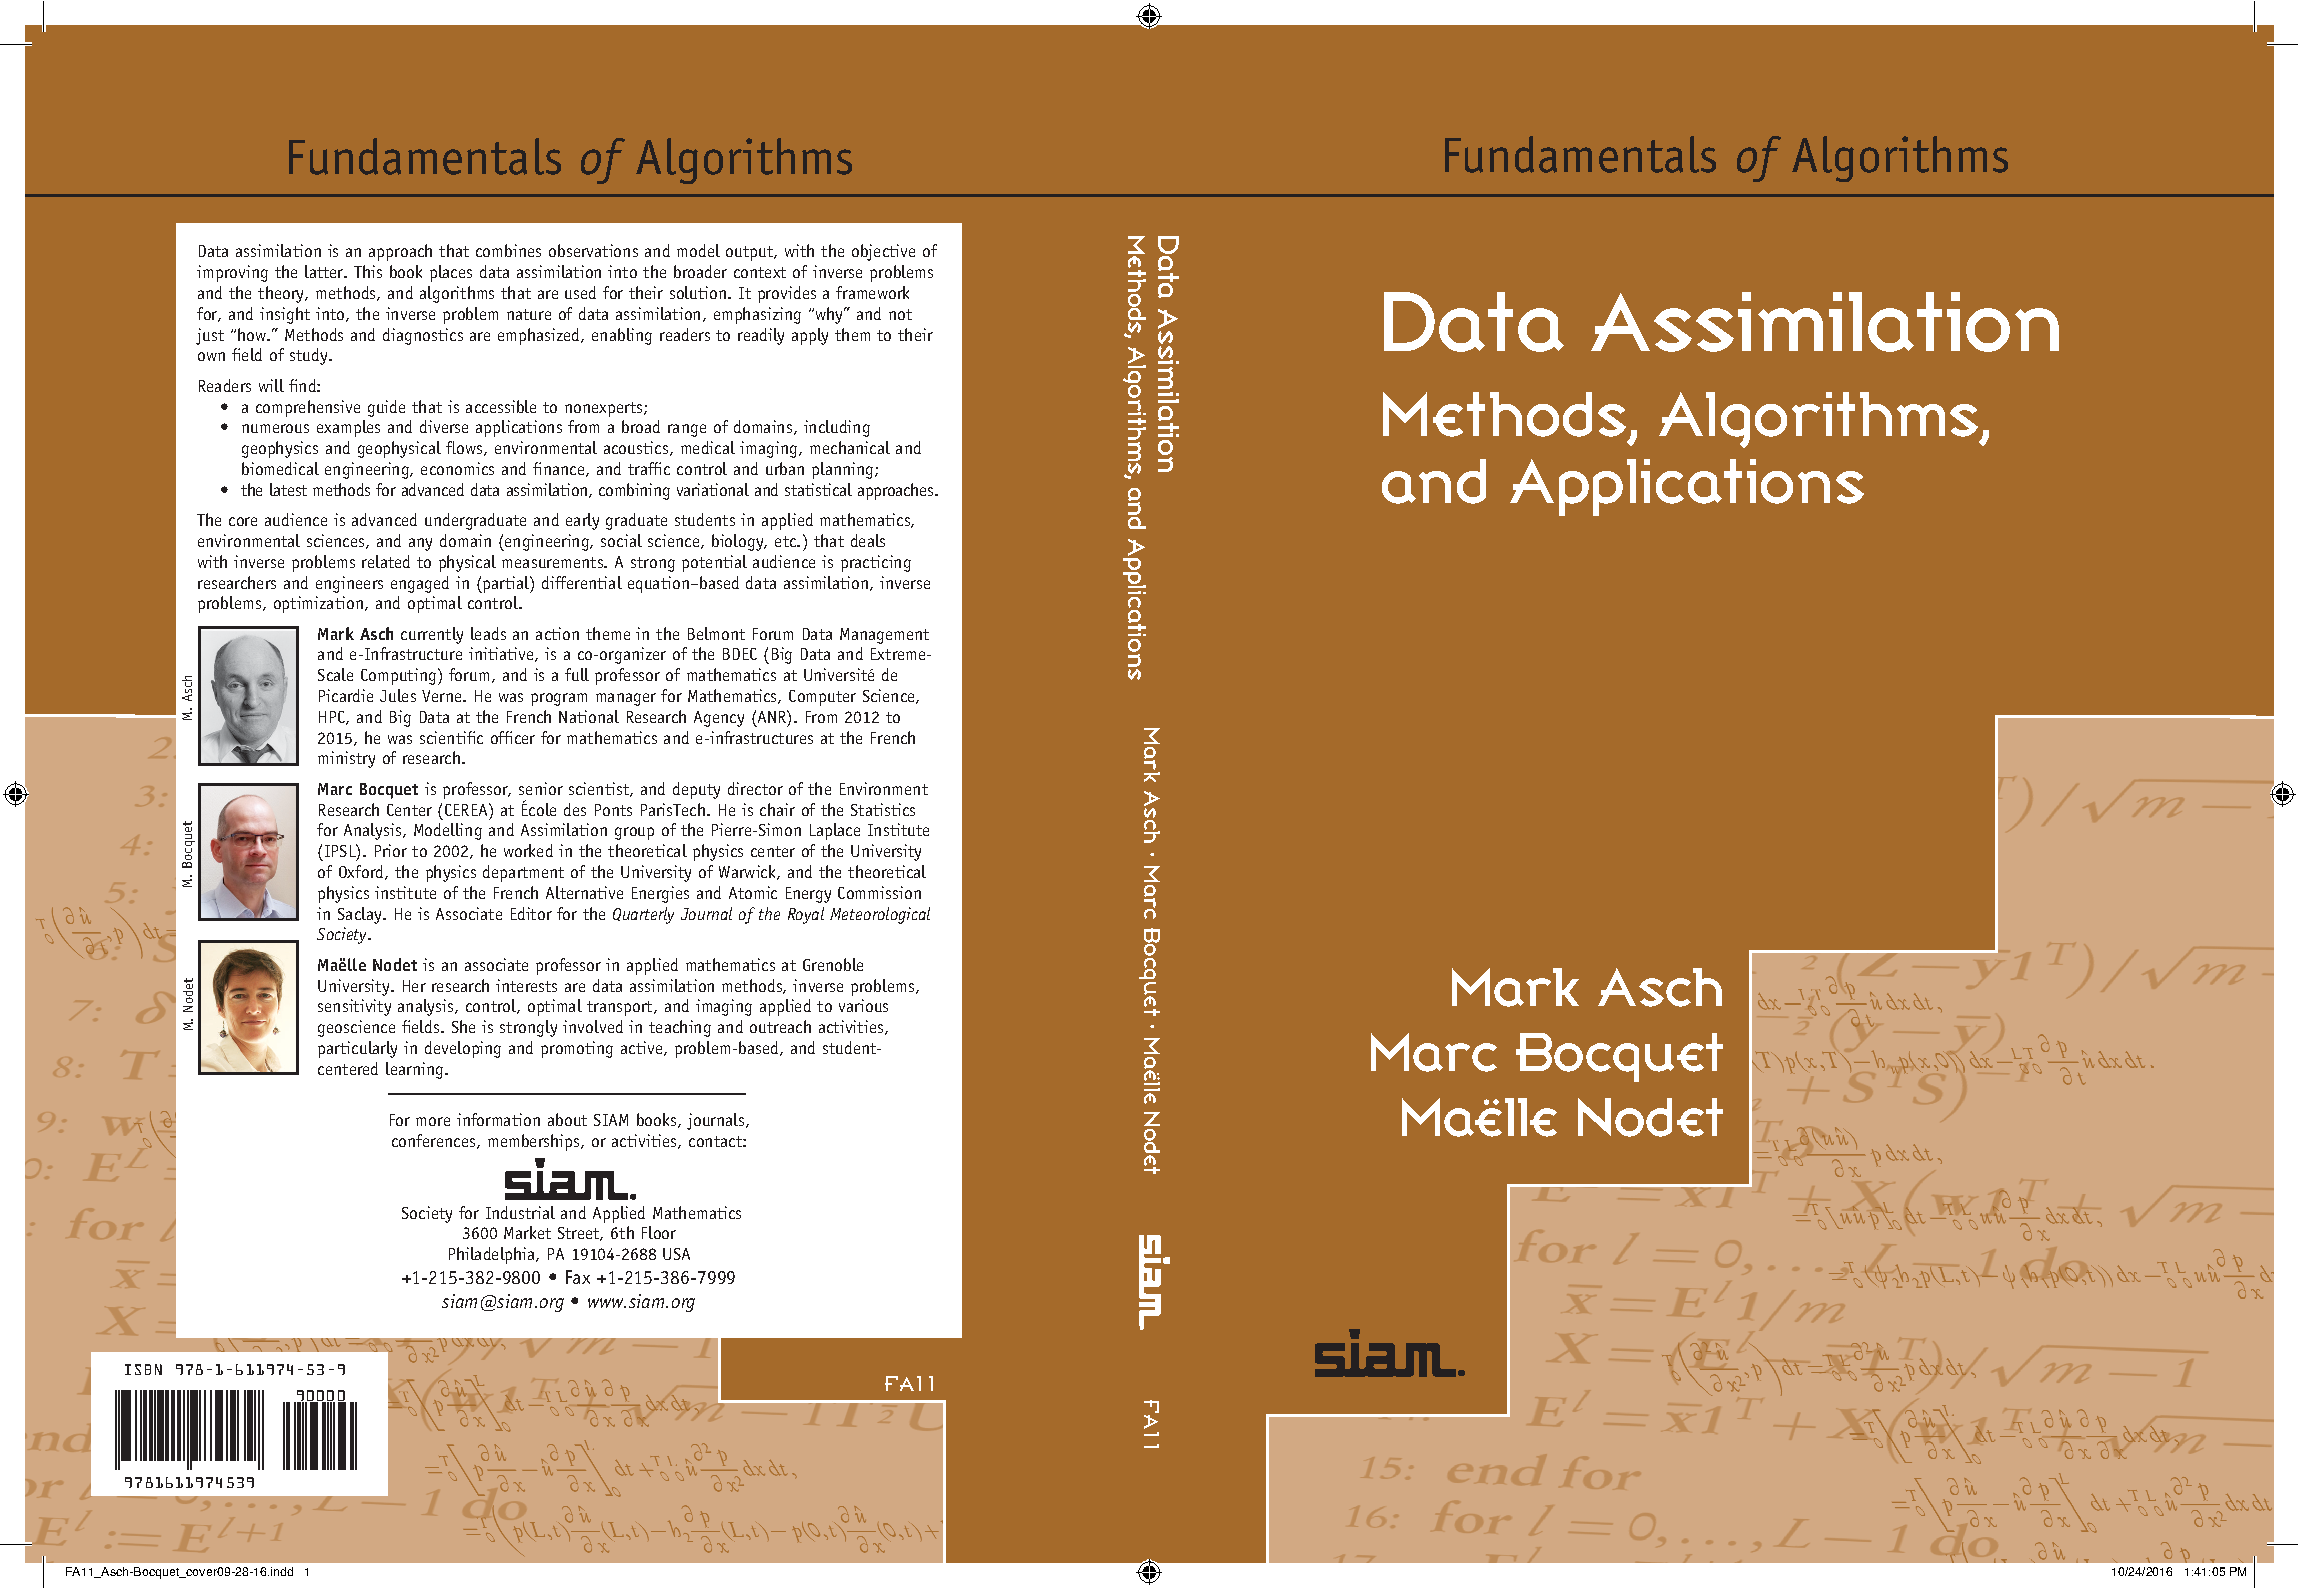
\includegraphics[width=0.8\textwidth]{graphics/FA11_Asch-Boucquet_cover10-24-16}
\par\end{center}

\begin{center}
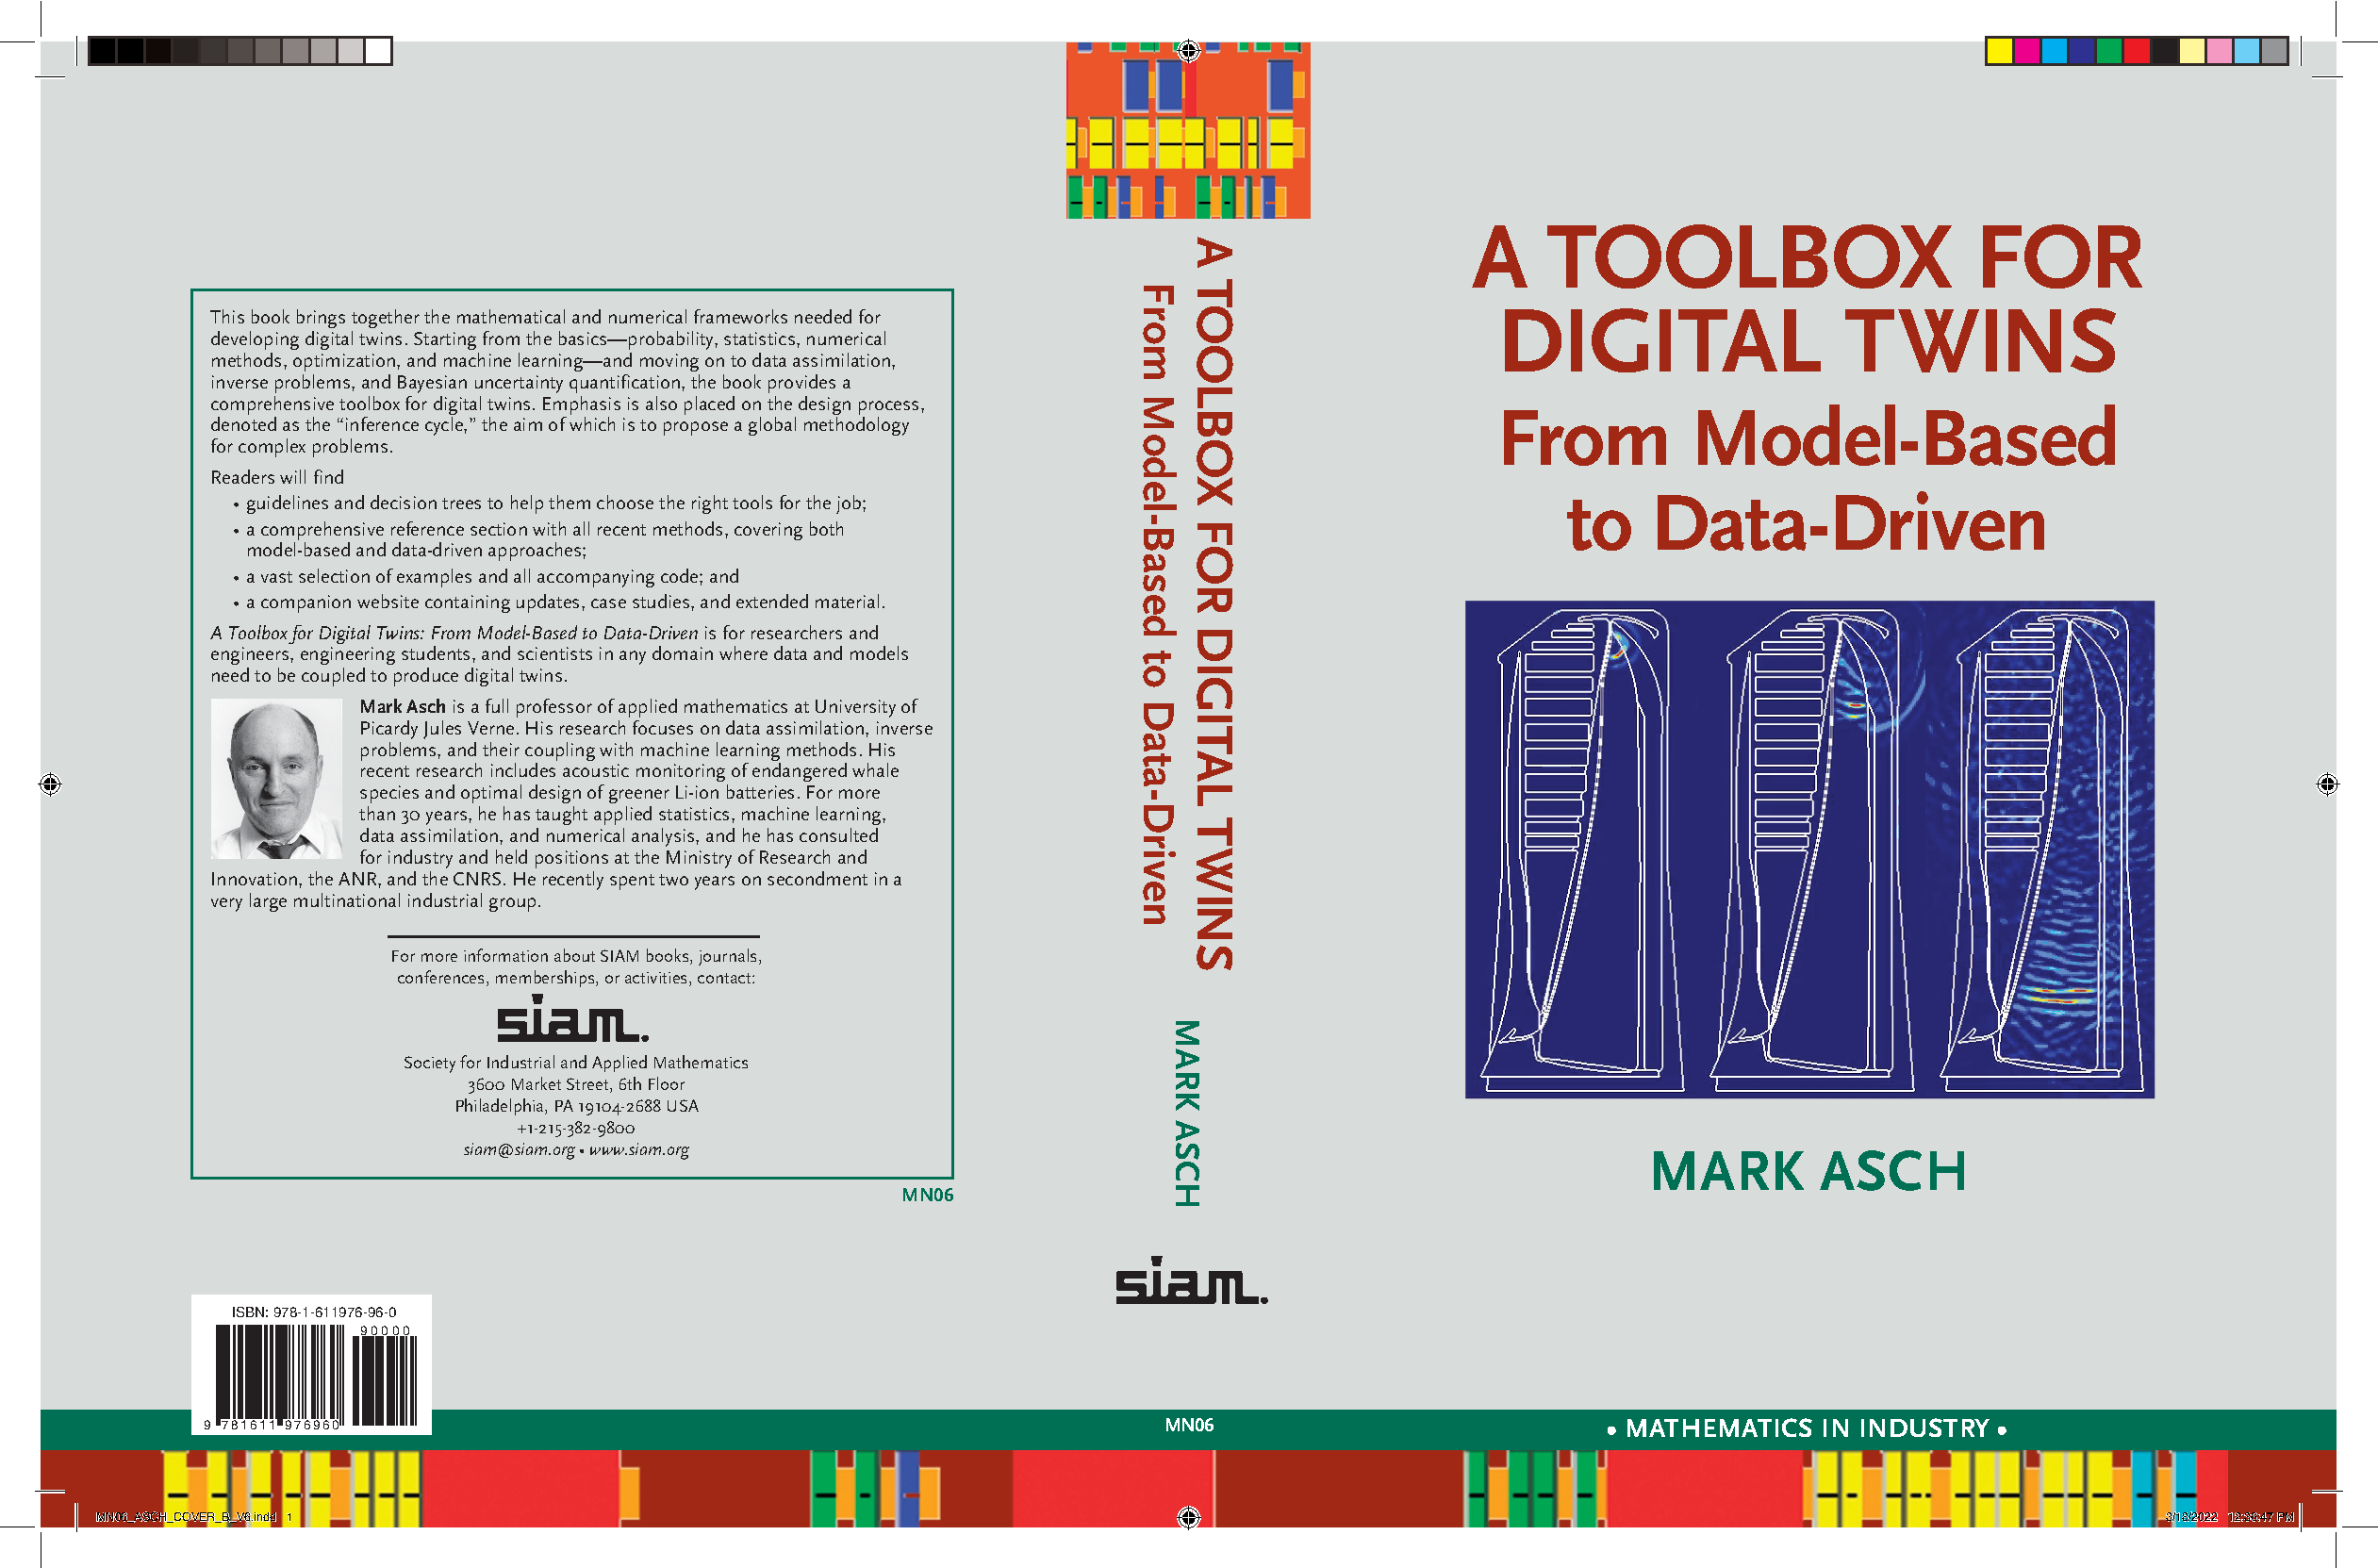
\includegraphics[width=0.8\textwidth]{graphics/MN06_ASCH_COVER_B_V6}
\par\end{center}

\foilhead{$\;$}

\vfill{}

\begin{center}
{\Large\textbf{\textcolor{blue}{ADJOINT METHOD FOR INVERSE PROBLEMS}}}{\Large\par}
\par\end{center}

\vfill{}


\foilhead{Adjoint Methods (I)}
\begin{itemize}
\item A very \textcolor{magenta}{general approach} for solving inverse problems...
including \textcolor{magenta}{Machine Learning!}
\item \textcolor{magenta}{Variational DA }is based on an \textcolor{magenta}{adjoint
approach}.
\end{itemize}
\begin{center}
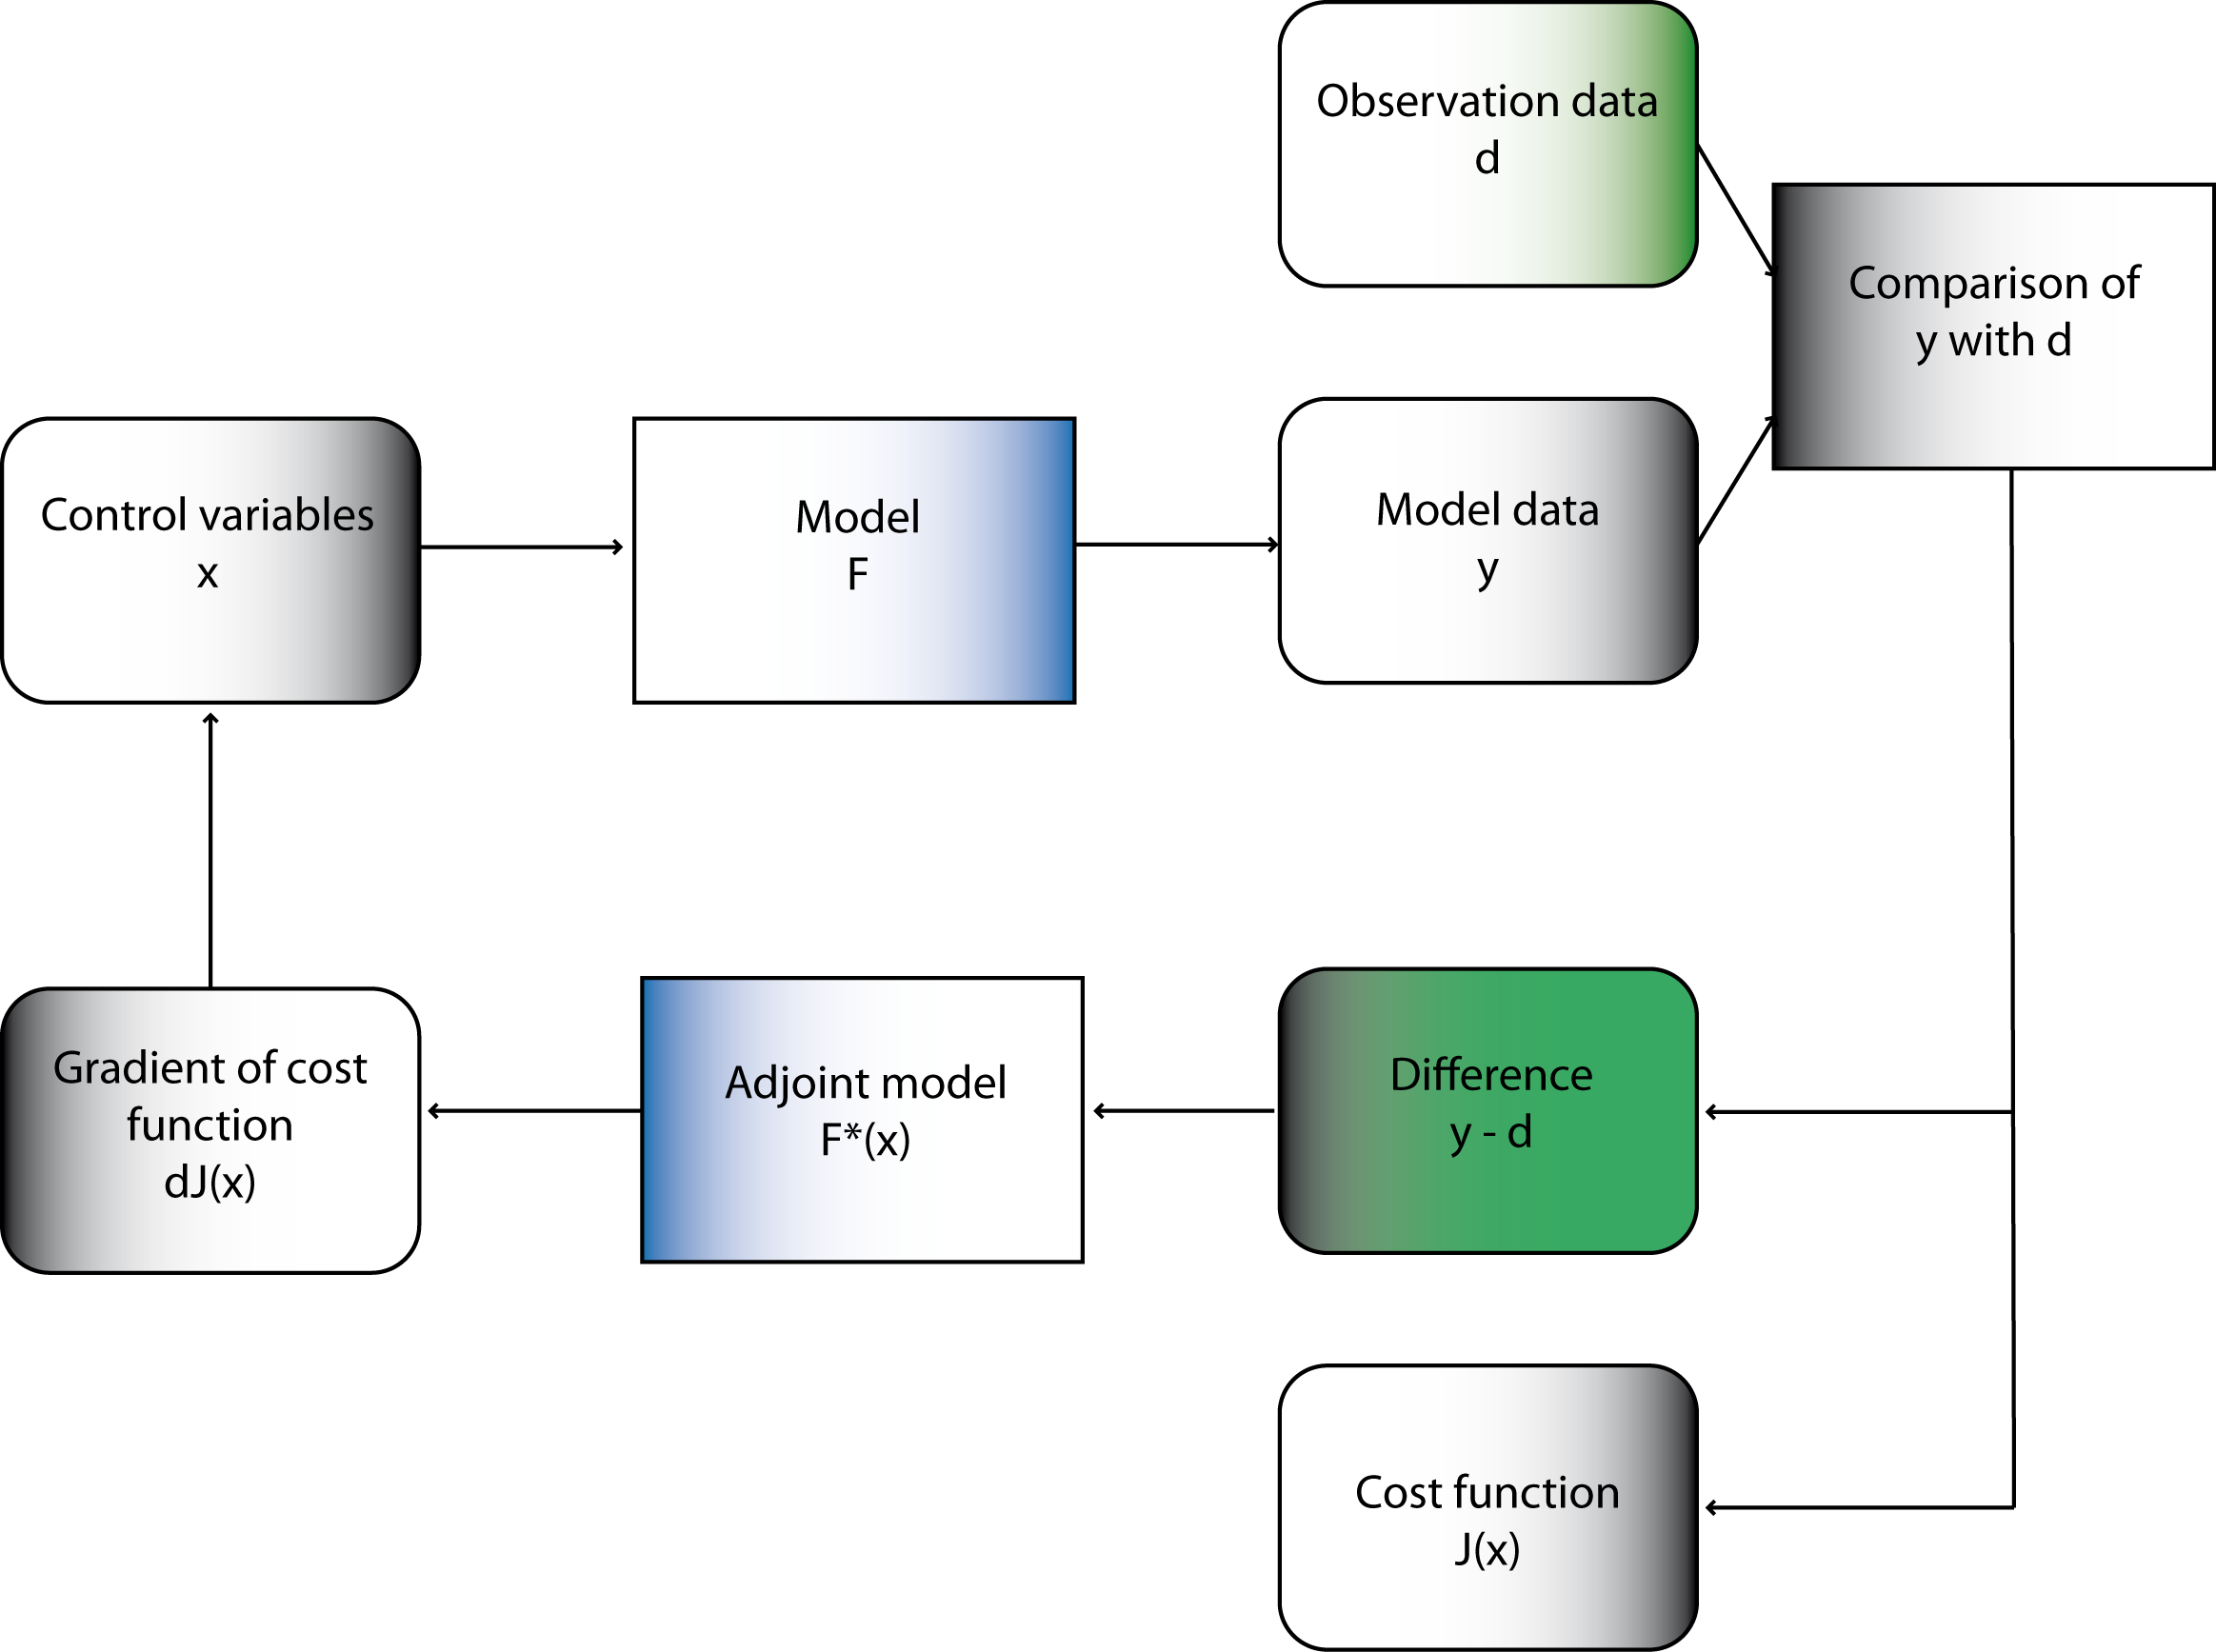
\includegraphics[width=1\textwidth]{graphics/adjoint}
\par\end{center}

\foilhead{Adjoint Methods (II) - definition}
\begin{defn}
{\large\textsl{\textcolor{red}{An }}}{\large\textbf{\textsl{\textcolor{red}{\emph{adjoint
method}}}}}{\large\textsl{\textcolor{red}{{} is a general mathematical
technique, based on variational calculus, that enables the computation
of the gradient of an objective, or cost functional with respect to
the model parameters in a very efficient manner.}}}{\large\par}
\end{defn}

\foilhead{Adjoint Methods (III) - continuous formulation}
\begin{itemize}
\item Let $\mathbf{u}(\mathbf{x},t)$ be the state of a \textit{\textcolor{magenta}{dynamical
system}} whose behavior depends on model parameters $\mathbf{m}(\mathbf{x},t)$
and is described by a differential operator equation 
\[
\mathbf{L}(\mathbf{u},\mathbf{m})=\mathbf{f},
\]
where $\mathbf{f}(\mathbf{x},t)$ represents external forces. 
\item Define a \textit{\textcolor{magenta}{cost function}} $J(\mathbf{m})$
as an energy functional\footnote{A functional is a generalization of a function. The functional depends
on functions, whereas a function depends on variables. We then say
that a functional is mapping from a space of functions into the real
numbers. } or, more commonly, as a \textcolor{magenta}{misfit functional }that
quantifies the error ($L^{2}$-distance\footnote{The $L^{2}$-space is a Hilbert space of (measurable) functions that
are square-integrable (in Lebesgue sense).}) between the observation and the model prediction $\mathbf{u}(\mathbf{x},t;\mathbf{m}).$
For example, 
\[
J(\mathbf{m})=\int_{0}^{T}\int_{\Omega}\left(\mathbf{u}(\mathbf{x},t;\mathbf{m})-\mathbf{u}^{\mathrm{obs}}(\mathbf{x},t)\right)^{2}\,\mathrm{d}\mathbf{x}\:\mathrm{d}t,
\]
where $\mathbf{x}\in\Omega\subset\mathbb{R}^{n},\,n=1,2,3,$ and $0\le t\le T.$ 
\item Our \textcolor{magenta}{objective} is to choose the model parameters
$\mathbf{m}$ as a function of the observed output $\mathbf{u}^{\mathrm{obs}},$
such that the cost function $J(\mathbf{m})$ is \textcolor{magenta}{minimized}.
\item The minimization is most frequently performed by a gradient-based
method, the simplest of which is steepest gradient, though usually
some variant of a quasi-Newton approach is used\textemdash see {[}Asch2022,
Nocedal2016{]}. 
\item If we can obtain an expression for the gradient, then the minimization
will be considerably facilitated. 
\item This is the objective of the adjoint method that provides an \textbf{\textcolor{magenta}{explicit
formula for the gradient of $J(\mathbf{m}).$}}
\end{itemize}

\foilhead{Adjoint Methods (IV) - optimization formulation}
\begin{itemize}
\item Suppose we are given a (P)DE, 
\begin{equation}
F(\mathbf{u};\mathbf{m})=0,\label{eq:pde}
\end{equation}
where 
\begin{itemize}
\item $\mathbf{u}$ is the state vector, 
\item $\mathbf{m}$ is the parameter vector, and 
\item $F$ includes the partial differential operator $\mathbf{L},$ the
right-hand side (source) $\mathbf{f},$ boundary and initial conditions. 
\end{itemize}
\item Note that the components of $\mathbf{m}$ can appear as any combination
of
\begin{itemize}
\item coefficients in the equation, 
\item the source, 
\item or as components of the boundary/initial conditions. 
\end{itemize}
\item To solve this very general parameter estimation problem, we are given
a cost function $J(\mathbf{m};\mathbf{u}).$ 
\begin{itemize}
\item The constrained optimization problem is then 
\[
\begin{cases}
\mathrm{minimize}_{\mathbf{m}} & J\left(\mathbf{u}(\mathbf{m}),\mathbf{m}\right)\\
\mathrm{subject\,to} & F(\mathbf{u};\mathbf{m})=0,
\end{cases}
\]
where $J$ can depend on both $\mathbf{u}$ and on $\mathbf{m}$ explicitly
in the presence of eventual regularization terms.
\item Note:
\begin{itemize}
\item the constraint is a (partial) differential equation and
\item the minimization is with respect to a (vector) function. 
\end{itemize}
\item This type of optimization is the subject of \textcolor{magenta}{variational
calculus},\index{adjoint method!calculus of variations} a generalization
of classical calculus where differentiation is performed with respect
to a variable, not a function.
\end{itemize}
\item The\textcolor{magenta}{{} gradient} of $J$ with respect to $\mathbf{m}$
(also known as the \emph{sensitivity}) is then obtained by the \textcolor{magenta}{chain-rule},
\[
\nabla_{\mathbf{m}}J=\frac{\partial J}{\partial\mathbf{u}}\frac{\partial\mathbf{u}}{\partial\mathbf{m}}+\frac{\partial J}{\partial\mathbf{m}}.
\]

\begin{itemize}
\item The partial derivatives of $J$ with respect to $\mathbf{u}$ and
$\mathbf{m}$ are readily computed from the expression for $J,$ 
\item but the derivative of $\mathbf{u}$ with respect to $\mathbf{m}$
requires a potentially very large number of evaluations, corresponding
to the product of the dimensions of $\mathbf{u}$ and $\mathbf{m}$
that can both be very large. 
\end{itemize}
\item The adjoint method is a way to \textcolor{red}{avoid} calculating
all of these derivatives. 
\item We use the fact that if $F(\mathbf{u};\mathbf{m})=0$ everywhere,
then this implies that the total derivative of $F$ with respect to
$\mathbf{m}$ is equal to zero everywhere too. 
\item Differentiating the PDE (\ref{eq:pde}), we can thus write 
\[
\frac{\partial F}{\partial\mathbf{u}}\frac{\partial\mathbf{u}}{\partial\mathbf{m}}+\nabla_{\mathbf{m}}F=0.
\]
\item This can be solved for the untractable derivative of $\mathbf{u}$
with respect to $\mathbf{m},$ to give 
\[
\frac{\partial\mathbf{u}}{\partial\mathbf{m}}=-\left(\frac{\partial F}{\partial\mathbf{u}}\right)^{-1}\nabla_{\mathbf{m}}F
\]
assuming that the inverse of $\partial F/\partial{\mathbf{u}}$ exists. 
\item Substituting in the expression for the gradient of $J,$ we obtain
\begin{align*}
\nabla_{\mathbf{m}}J & =-\frac{\partial J}{\partial\mathbf{u}}\left(\frac{\partial F}{\partial\mathbf{u}}\right)^{-1}\nabla_{\mathbf{m}}F+\frac{\partial J}{\partial\mathbf{m}},\\
 & =\mathbf{p}\nabla_{\mathbf{m}}F+\frac{\partial J}{\partial\mathbf{m}}
\end{align*}
where 
\begin{itemize}
\item we have conveniently defined $\mathbf{p}$ as the solution of the
\textcolor{magenta}{\emph{adjoint equation}} 
\[
\left(\frac{\partial F}{\partial\mathbf{u}}\right)^{\T}\mathbf{p}=-\frac{\partial J}{\partial\mathbf{u}}.
\]
\end{itemize}
\end{itemize}

\foilhead{Adjoint Methods (V) - summing up}

In summary, we have a three-step procedure that combines a model-based
approach (through the PDE) with a data-driven approach (through the
cost function): 
\begin{enumerate}
\item Solve the \textcolor{magenta}{\emph{adjoint equation}} for the adjoint
state, $\mathbf{p}.$ 
\item Using the adjoint state, compute the \textcolor{magenta}{\emph{gradient}}
of the cost function $J.$ 
\item Using the gradient, solve the \textcolor{magenta}{\emph{optimization}}
problem to estimate the parameters $\mathbf{m}$ that \textcolor{magenta}{\emph{minimize
the mismatch}} between model and observations. 
\end{enumerate}
\noindent\shadowbox{\begin{minipage}[t]{1\columnwidth - 2\fboxsep - 2\fboxrule - \shadowsize}%
\textcolor{red}{This key result enables us to compute the desired
gradient, $\nabla_{\mathbf{m}}J,$ without the explicit knowledge
of the variation of $\mathbf{u}.$} %
\end{minipage}}
\begin{itemize}
\item A number of {important remarks} can be made.
\begin{enumerate}
\item We obtain \textcolor{magenta}{\emph{explicit}}\textcolor{magenta}{{}
}formulas\textemdash in terms of the adjoint state\textemdash for
the gradient with respect to each/any model parameter. Note that this
has been done in a completely general setting, without any restrictions
on the operator ${F}$ or on the model parameters $\mathbf{m}.$ 
\item The \textcolor{magenta}{\emph{computational cost}}\textcolor{magenta}{{}
}is one solution of the adjoint equation which is usually of the same
order as (if not identical to) the direct equation, but with a reversal
of time. {Note that for nonlinear equations this may not be the case
and one may require four or five times the computational effort.} 
\item The \textcolor{magenta}{\emph{variation}} (G�teaux derivative) of
${F}$ with respect to the model parameters $\mathbf{m}$ is, in general,
straightforward to compute. 
\item We have not explicitly considered boundary (or initial) conditions
in the above, general approach. In real cases, these are potential
sources of difficulties for the use of the adjoint approach\textemdash the
\emph{discrete adjoint} can provide a way to overcome this hurdle. 
\item For complete mathematical rigor, the above development should be performed
in an appropriate \textcolor{magenta}{\emph{Hilbert space}}\textcolor{magenta}{{}
}setting that guarantees the existence of all the inner products and
adjoint operators. The interested reader could consul {[}Troltzsch2010{]}.
\item In many real problems, the optimization of the misfit functional leads
to \textcolor{magenta}{\emph{multiple local minima}} and often to
very ``flat'' cost functions. These are hard problems for gradient-based
optimization methods. These difficulties can be (partially) overcome
by a panoply of tools: 
\begin{enumerate}
\item \textcolor{magenta}{\emph{Regularization}}\index{regularization}
terms can alleviate the non-uniqueness problem. 
\item \textcolor{magenta}{\emph{Rescaling}} the parameters and/or variables
in the equations can help with the ``flatness.'' This technique
is often employed in numerical optimization.
\item \textcolor{magenta}{\emph{Hybrid}} algorithms, that combine stochastic
and deterministic optimization (e.g., Simulated Annealing), can be
used to avoid local minima.
\item Judicious use of \textcolor{magenta}{machine learning} techniques
and methods.
\end{enumerate}
\item When measurement and modeling errors can be modeled by Gaussian distributions
and a background (prior) solution exists, the objective function may
be generalized by including suitable \textcolor{magenta}{\emph{covariance
matrices}}\textcolor{magenta}{.} This is the approach employed systematically
in data assimilation\textemdash see below.
\end{enumerate}
\end{itemize}

\foilhead{Adjoint Methods (VI) - Examples}
\begin{itemize}
\item We will now present a series of examples where we apply the adjoint
approach to increasingly complex\textcolor{magenta}{{} cases of inverse
problems}, for which we have
\begin{itemize}
\item a cost/mismatch function to minimze
\item subject to the constraint of a (P)DE. 
\end{itemize}
\item There are \textcolor{magenta}{two alternative methods} for the derivation
of the adjoint equation:
\begin{itemize}
\item the \textcolor{magenta}{Lagrange multiplier} approach \index{Lagrange multiplier}\index{Lagrange multiplier|see {adjoint method}} 
\item and the \textcolor{magenta}{tangent linear model} (TLM)\index{tangent linear model|see {adjoint method}}
approach. 
\end{itemize}
\item After seeing the two in action, the reader can adopt the one that
suits her/him best. 
\item Note that the Lagrangian approach supposes that we perturb the sought
for parameters and is thus not applicable to inverting for constant-valued
parameters, in which case we must resort to the tangent linear model
approach.
\end{itemize}

\foilhead{$\;$}

\vfill{}

\begin{center}
{\Large\textbf{\textcolor{blue}{ADJOINT METHOD EXAMPLES}}}{\Large\par}
\par\end{center}

\vfill{}


\foilhead[-0.5in]{Example: TLM Adjoint Method for Parameter Identification}
\begin{itemize}
\item Consider the \textcolor{magenta}{parameter identification problem}
for the 1D \textcolor{magenta}{convection-diffusion equation}\index{convection-diffusion equation},
\begin{equation}
\left\{ \begin{aligned} & -bu''(x)+cu'(x)=f(x),\quad0<x<1,\\
 & u(0)=0,\;u(1)=0,
\end{aligned}
\right.\label{eq:cnvdif-2}
\end{equation}
where
\begin{itemize}
\item $f$ is a given function 
\item $b$ and $c$ are the unknown (constant) parameters that we seek to
identify
\item using observations of $u(x)$ on $[0,1].$ 
\end{itemize}
\item The \textcolor{magenta}{least-squares error cost function} is 
\[
J(b,c)=\frac{1}{2}\int_{0}^{1}\left(u(x)-u^{\mathrm{obs}}(x)\right)^{2}\mathrm{d}x.
\]
\item We calculate its \textcolor{magenta}{gradient} by introducing the
\textcolor{magenta}{\emph{tangent linear model}}\index{tangent linear model}.
\begin{itemize}
\item Perturbing the cost function by a small perturbation in the direction
$\alpha$ with respect to the two parameters gives 
\begin{align*}
J(b+\alpha\delta b,c+\alpha\delta c)-J(b,c)\\
=\frac{1}{2}\int_{0}^{1}\left(\tilde{u}-u^{\mathrm{obs}}\right)^{2}-\left(u-u^{\mathrm{obs}}\right)^{2}\mathrm{d}x,
\end{align*}
where
\begin{itemize}
\item $\tilde{u}=u_{b+\alpha\delta b,c+\alpha\delta c}$ is the perturbed
solution and
\item $u=u_{b,c}$ is the unperturbed one. 
\end{itemize}
\item Expanding and rearranging, we obtain 
\begin{align*}
J(b+\alpha\delta b,c+\alpha\delta c)-J(b,c)\\
=\frac{1}{2}\int_{0}^{1}\left(\tilde{u}+u-2u^{\mathrm{obs}}\right)\left(\tilde{u}-u\right)\mathrm{d}x.
\end{align*}
\item Now we divide by $\alpha$ on both sides of the equation and \textcolor{magenta}{pass
to the limit} $\alpha\rightarrow0,$ to obtain the \textcolor{magenta}{directional
derivative }(which is the derivative with respect to the parameters,
in the direction of the perturbations), 
\begin{equation}
\hat{J}\left[b,c\right](\delta b,\delta c)=\int_{0}^{1}\left(u-u^{\mathrm{obs}}\right)\hat{u}\,\mathrm{d}x,\label{eq:dirder-1}
\end{equation}
where 
\begin{itemize}
\item we have defined 
\begin{align*}
\hat{u} & =\lim_{\alpha\rightarrow0}\frac{\tilde{u}-u}{\alpha},\\
\hat{J}\left[b,c\right](\delta b,\delta c) & =\lim_{\alpha\rightarrow0}\frac{J(b+\alpha\delta b,c+\alpha\delta c)-J(b,c)}{\alpha}
\end{align*}
\item and we have moved the limit under the integral sign. 
\end{itemize}
\item Now use this definition to find the equation satisfied by $\hat{u}.$ 
\begin{itemize}
\item We have the perturbed equation, 
\[
\left\{ \begin{aligned} & -(b+\alpha\delta b)\tilde{u}''+(c+\alpha\delta c)\tilde{u}'=f,\\
 & \tilde{u}(0)=0,\;\tilde{u}(1)=0,
\end{aligned}
\right.
\]
and the given model (\ref{eq:cnvdif-2}), 
\[
\left\{ \begin{aligned} & -bu''+cu'=f,\\
 & u(0)=0,\;u(1)=0.
\end{aligned}
\right.
\]
\item Then, subtracting these two equations and \textcolor{magenta}{passing
to the limit }(using the definition of $\hat{u}$) we obtain 
\[
\left\{ \begin{aligned} & -b\hat{u}''-(\delta b)u''+c\hat{u}'+(\delta c)u'=0,\\
 & \hat{u}(0)=0,\;\hat{u}(1)=0.
\end{aligned}
\right.
\]
\end{itemize}
\item Regrouping terms, we can now define the \textcolor{magenta}{\emph{tangent
linear model}} 
\begin{equation}
\left\{ \begin{aligned} & -b\hat{u}''+c\hat{u}'=(\delta b)u''-(\delta c)u',\\
 & \hat{u}(0)=0,\;\hat{u}(1)=0.
\end{aligned}
\right.\label{eq:ltm-1}
\end{equation}
\item We want to be able to reformulate the directional derivative (\ref{eq:dirder-1}),
in order to obtain a calculable expression for the gradient. 
\item So we multiply the tangent linear model (\ref{eq:ltm-1}) by a variable
$p$ and we \textcolor{magenta}{integrate twice by parts}, transferring
derivatives from $\hat{u}$ onto $p$: 
\begin{align*}
-b\int_{0}^{1}\hat{u}''p\,\mathrm{d}x+c\int_{0}^{1}\hat{u}'p\,\mathrm{d}x\\
=\int_{0}^{1}\left((\delta b)u''\,\mathrm{d}x-(\delta c)u'\right)p\,\mathrm{d}x,
\end{align*}
which gives (term-by-term) 
\begin{eqnarray*}
\int_{0}^{1}\hat{u}''p\,\mathrm{d}x & = & \left[\hat{u}'p\right]_{0}^{1}-\int_{0}^{1}\hat{u}'p'\,\mathrm{d}x\\
 & = & \left[\hat{u}'p-\hat{u}p'\right]_{0}^{1}+\int_{0}^{1}\hat{u}p''\,\mathrm{d}x\\
 & = & \hat{u}'(1)p(1)-\hat{u}'(0)p(0)+\int_{0}^{1}\hat{u}p''\,\mathrm{d}x
\end{eqnarray*}
and 
\begin{eqnarray*}
\int_{0}^{1}\hat{u}'p\,\mathrm{d}x & = & \left[\hat{u}p\right]_{0}^{1}-\int_{0}^{1}\hat{u}p'\,\mathrm{d}x\\
 & = & -\int_{0}^{1}\hat{u}p'\,\mathrm{d}x.
\end{eqnarray*}
\item Putting these results together, we have 
\begin{align*}
-b\left(\hat{u}'(1)p(1)-\hat{u}'(0)p(0)+\int_{0}^{1}\hat{u}p''\right)\\
+c\left(-\int_{0}^{1}\hat{u}p'\right)\\
=\int_{0}^{1}\left((\delta b)u''-(\delta c)u'\right)p
\end{align*}
or, grouping terms, 
\begin{align}
\int_{0}^{1}\left(-bp''-cp'\right)\hat{u}\label{eq:intp-1}\\
=b\hat{u}'(1)p(1)-b\hat{u}'(0)p(0)\\
+\int_{0}^{1}\left((\delta b)u''-(\delta c)u'\right)p.
\end{align}
\item Now, in order to get rid of \emph{all} the terms in $\hat{u}$ in
this expression, we impose that $p$ must satisfy \emph{the adjoint
model} 
\begin{equation}
\left\{ \begin{aligned} & -bp''-cp'=(u-u^{\mathrm{obs}}),\\
 & p(0)=0,\;p(1)=0.
\end{aligned}
\right.\label{eq:adjode-1}
\end{equation}
\item Integrating (\ref{eq:adjode-1}) and using the expression (\ref{eq:intp-1}),
we obtain 
\begin{align*}
\int_{0}^{1}(u-u^{\mathrm{obs}})\hat{u}\\
=\int_{0}^{1}\left(-bp''-cp'\right)\hat{u}\\
=(\delta b)\left(\int_{0}^{1}pu''\right)+(\delta c)\left(-\int_{0}^{1}pu'\right).
\end{align*}
\item We recognize, in the last two terms, \textcolor{magenta}{the $L^{2}$
inner product}, which enables us, based on the definition of the \textcolor{magenta}{directional
derivative} as the inner product between the gradient and the parameter
perturbations, 
\[
\delta J\doteq\nabla_{\mathbf{m}}J\delta\mathbf{m},
\]
to finally write an explicit expression for the gradient, based on
(\ref{eq:dirder-1}), 
\[
\nabla J(b,c)=\left(\int_{0}^{1}pu''\mathrm{d}x,-\int_{0}^{1}pu'\mathrm{d}x\right)^{\T},
\]
\end{itemize}
\item or, separating the two components, 
\begin{eqnarray}
\nabla_{b}J(b,c) & = & \int_{0}^{1}pu''\mathrm{d}x,\label{eq:gradJb}\\
\nabla_{c}J(b,c) & = & -\int_{0}^{1}pu'\mathrm{d}x.\label{eq:gradJc}
\end{eqnarray}
\item Thus, in this example, to \textcolor{magenta}{compute the gradient
of the least-squares error cost function}, we must:
\begin{itemize}
\item \textcolor{magenta}{solve the direct equation} (\ref{eq:cnvdif-2})
for $u$ and derive $u'$ and $u''$ from the solution, using some
form of numerical differentiation (if we solved with finite differences),
or differentiating the shape functions (if we solved with finite elements); 
\item \textcolor{magenta}{solve the adjoint equation} (\ref{eq:adjode-1})
for $p$ (using the same solver\footnote{This is not true when we use a \emph{discrete} adjoint approach\textemdash see
Section \ref{sec:disc_adj}} that we used for $u$); 
\item \textcolor{magenta}{compute the two terms of the gradient}, (\ref{eq:gradJb})
and (\ref{eq:gradJc}), using any suitable numerical integration scheme. 
\end{itemize}
\item \textbf{Conclusion}:
\begin{itemize}
\item Thus for the \textcolor{magenta}{additional cost }of one solution
of the adjoint model (\ref{eq:adjode-1}) plus a numerical integration,
we can compute the gradient of the cost function with respect to either
one or both of the unknown parameters. 
\item It is now a relatively easy task to find (numerically) the optimal
values of $b$ and $c$ that minimize $J$ by a suitable \textcolor{magenta}{descent
algorithm}, for example a quasi-Newton methods;
\item Note that this problem can be modified to treat the case where the
observation is at one end-point, together with a discrete number of
points in the interval. 
\begin{itemize}
\item In this case, the corresponding boundary condition must be of Neumann
or mixed type, and the cost function needs to be modified, becoming
a sum of the squared mismatches over the discrete observation points. 
\item The adjoint boundary conditions and right-hand side will also be modified,
but the expressions for the gradients will remain exactly the same.
\end{itemize}
\end{itemize}
\end{itemize}

\foilhead[-0.5in]{Example: Lagrangian Adjoint Method for Parameter Identification}
\begin{itemize}
\item We now consider a variant of the \textcolor{magenta}{convection-diffusion}\index{convection-diffusion equation}
example, where the \textcolor{magenta}{diffusion coefficient is spatially
varying}. 
\begin{itemize}
\item This model is closer to many physical situations, where the medium
is not homogeneous and we have zones with differing diffusive properties. 
\end{itemize}
\item The system is now
\end{itemize}
\begin{equation}
\left\{ \begin{aligned} & -\left(a(x)u'(x)\right)'-u'(x)=q(x),\quad0<x<1,\\
 & u(0)=0,\;u(1)=0.
\end{aligned}
\right.\label{eq:cnvdif-1}
\end{equation}

\begin{itemize}
\item with the cost function
\[
J[a]=\frac{1}{2}\int_{0}^{1}\left(u(x)-u^{\mathrm{obs}}(x)\right)^{2}\,\dd x,
\]
where $u^{\mathrm{obs}}(x)$ denotes the observations on $\left[0,1\right].$ 
\item We now introduce an alternative approach for deriving the gradient,
based on the \textcolor{magenta}{Lagrangian} (or variational formulation). 
\item Let the cost function 
\begin{align*}
J^{*}[a,p] & =\frac{1}{2}\int_{0}^{1}\left(u(x)-u^{\mathrm{obs}}(x)\right)^{2}\,\dd x\\
 & +\int_{0}^{1}p\left(-\left(au'\right)'-u'-q\right)\dd x,
\end{align*}
noting that 
\begin{itemize}
\item the second integral is zero when $u$ is a solution of (\ref{eq:cnvdif-1}) 
\item and that the adjoint variable, $p,$ can be considered here to be
a Lagrange multiplier\index{Lagrange multiplier} function.
\end{itemize}
\item We begin by taking the variation of $J^{*}$ with respect to its variables,
$a$ and $p,$ 
\begin{align*}
\delta J^{*} & =\int_{0}^{1}\left(u-u^{\mathrm{obs}}\right)\delta u\,\dd x\\
 & +\int_{0}^{1}\delta p\overbrace{\left(-\left(au'\right)'-u'-q\right)}^{=\,0}\dd x\\
 & +\int_{0}^{1}p\left[\left(-\delta a\,u'-a\,\delta u'\right)'\right].
\end{align*}
\item Now the strategy is to \textcolor{magenta}{``kill terms'' }by imposing
suitable, well-chosen conditions on $p.$ 
\begin{itemize}
\item This is achieved by i\textcolor{magenta}{ntegrating by parts} and
then defining the \textcolor{magenta}{adjoint equation} and boundary
conditions on $p$ as follows: 
\begin{eqnarray*}
\delta J^{*} & = & \int_{0}^{1}\left[(u-u^{\mathrm{obs}})+p'-(ap')'\right]\delta u\,\dd x\\
 &  & +\int_{0}^{1}\delta a\,u'p'\dd x\\
 &  & +\left[-p(\delta u+u'\delta a+a\delta u')+p'a\delta u\right]_{0}^{1}\\
 & = & \int_{0}^{1}\delta a\,u'p'\dd x,
\end{eqnarray*}
where 
\begin{itemize}
\item we have used the zero boundary conditions on $\delta u$ 
\item and assumed that the following adjoint system must be satisfied by
$p$: 
\begin{equation}
\left\{ \begin{aligned} & -\left(ap'\right)'+p'=-(u-u^{\mathrm{obs}}),\quad0<x<1,\\
 & p(0)=0,\;p(1)=0.
\end{aligned}
\right.\label{eq:cnvdif-1-1}
\end{equation}
\end{itemize}
\item And, as before, based on the key result relating the variation to
the gradient, we are left with an \textcolor{magenta}{explicit expression
for the gradient}, \textcolor{red}{
\[
\nabla_{a(x)}J^{*}=u'p'.
\]
}
\end{itemize}
\item Thus with 
\begin{itemize}
\item one solution of the direct system (\ref{eq:cnvdif-1}) plus 
\item one solution of the adjoint system (\ref{eq:cnvdif-1-1}), we recover
the gradient of the cost function with respect to the sought for diffusion
coefficient, $a(x).$
\end{itemize}
\end{itemize}

\foilhead[-0.5in]{Example: Lagrangian Adjoint Method for Diffusion Equation}
\begin{itemize}
\item The natural extension of the ordinary differential equations seen
above is the initial-boundary-value problem known as the \textcolor{magenta}{diffusion
equation}, 
\begin{eqnarray*}
%
\frac{\partial u}{\partial t}-\nabla\cdot(\nu\nabla u)=0, & \quad x\in(0,L), & t>0,\\
u(x,0)=u_{0}(x),\text{\,\ } & u(0,t)=0, & u(L,t)=\eta(t).%{array}
\end{eqnarray*}
\item This equation has multiple origins emanating from different physical
situations. 
\begin{itemize}
\item The most common application is \textcolor{magenta}{particle diffusion},
where $u$ is a concentration and $\nu$ is a diffusion coefficient. 
\item Then there is \textcolor{magenta}{heat diffusion}, for which $u$
is a temperature and $\nu$ is a thermal conductivity. 
\item The equation is also found in finance, being closely related to the
Black-Scholes model\index{Black-Scholes equation}. 
\item Another important application is \textcolor{magenta}{population dynamics}. 
\item These diverse application fields, and hence the diffusion equation,
give rise to a number of \textcolor{magenta}{inverse and data assimilation
problems}.
\end{itemize}
\item A variety of different controls can be applied to this system:
\begin{itemize}
\item \textcolor{magenta}{\emph{internal}}\textcolor{magenta}{{} }control,
$\nu(x)$: this is the parameter identification problem, also known
as tomography\index{tomography}; 
\item \textcolor{magenta}{\emph{initial}} control, $\xi(x)=u_{0}(x)$: this
is a source detection IP or DA problem; 
\item \textcolor{magenta}{\emph{boundary}} control, $\eta(t)=u(L,t)$: this
is the ``classical'' boundary control problem, also a parameter
identification IP. 
\end{itemize}
\item As above, we can define the mismatch/L2\textcolor{magenta}{\emph{
cost function}}, 
\[
J[\nu,\xi,\eta]=\frac{1}{LT}\int_{0}^{T}\int_{0}^{L}\left(u-u^{\mathrm{obs}}\right)^{2}\,\mathrm{d}x\,\mathrm{d}t,
\]
which is now a space-time multiple integral, and its related \textcolor{magenta}{\noun{Lagrangian}},
\begin{align*}
J^{*} & =\frac{1}{LT}\int_{0}^{T}\!\!\int_{0}^{L}\left(u-u^{\mathrm{obs}}\right)^{2}\,\mathrm{d}x\,\mathrm{d}t\\
 & +\frac{1}{LT}\int_{0}^{T}\!\!\int_{0}^{L}p\left[u_{t}-(\nu u_{x})_{x}\right]\,\mathrm{d}x\,\mathrm{d}t.
\end{align*}
\item Now take the variation of $J^{*},$ 
\begin{eqnarray*}
\delta J^{*} & = & \frac{1}{LT}\int_{0}^{T}\!\!\int_{0}^{L}2(u-u^{\mathrm{obs}})\delta u\,\mathrm{d}x\,\mathrm{d}t\\
 &  & +\frac{1}{LT}\int_{0}^{T}\!\!\int_{0}^{L}\delta p\overbrace{\left[u_{t}-(\nu u_{x})_{x}\right]}^{=\,0}\,\mathrm{d}x\,\mathrm{d}t\\
 &  & +\frac{1}{LT}\int_{0}^{T}\!\!\int_{0}^{L}p\left[\delta u_{t}-(\delta\nu\,u_{x}+\nu\delta u_{x})_{x}\right]\,\mathrm{d}x\,\mathrm{d}t,
\end{eqnarray*}
and perform \textcolor{magenta}{integration by parts }to obtain 
\begin{align}
\delta J^{*} & =\frac{1}{LT}\int_{0}^{T}\!\!\int_{0}^{L}\delta\nu\,u_{x}p_{x}\,\mathrm{d}x\,\mathrm{d}t\ \label{eq:dJstar0}\\
 & -\frac{1}{LT}\int_{0}^{L}p\,\left.\delta u\right|_{t=0}\mathrm{d}x\\
 & +\frac{1}{LT}\int_{0}^{T}p\,\left.\delta\eta\right|_{x=L}\mathrm{d}t,
\end{align}
where we have defined the\textcolor{magenta}{{} adjoint equation} as
\begin{eqnarray*}
%
 &  & \frac{\partial p}{\partial t}+\nabla\cdot(\nu\nabla u)=2(u-u^{\mathrm{obs}}),\quad x\in(0,L),\quad t>0,\\
 &  & p(0,t)=0,\quad p(L,t)=0,\\
 &  & p(x,T)=0.%{array}
\end{eqnarray*}
\item As before, this equation is of the same type as the original diffusion
equation, but must be solved \textcolor{magenta}{backwards in time}. 
\item Finally, from (\ref{eq:dJstar0}) we can pick off each of the three
desired \textcolor{magenta}{terms of the gradient}, \textcolor{red}{
\begin{eqnarray*}
\nabla_{\nu(x)}J^{*} & = & \frac{1}{T}\int_{0}^{T}u_{x}p_{x}\,\mathrm{d}t,\\
\nabla_{\left.u\right|_{t=0}}J^{*} & = & -\left.p\right|_{t=0},\\
\nabla_{\left.\eta\right|_{x=L}}J^{*} & = & \left.p\right|_{x=L}.
\end{eqnarray*}
}
\item \textbf{\textcolor{magenta}{Conclusion}}: 
\begin{itemize}
\item Once again, at the expense of a single (backward) solution of the
adjoint equation, we obtain explicit expressions for the gradient
of the cost function with respect to each of the three control variables.
T
\item his is quite remarkable and completely avoids ``brute force'' or
exhaustive minimization, though, as mentioned earlier, we only have
the guarantee to find a local minimum. 
\item However, if we have a good starting guess that is usually obtained
from historical or other ``physical'' knowledge of the system, we
are sure to arrive at a good (or at least, better) minimum.
\end{itemize}
\end{itemize}
\selectlanguage{french}%

\foilhead[-0.5in]{\textcolor{blue}{Adjoint Example (III) : Nonlinear PDE (Burgers)}}
\begin{itemize}
\item Burgers Equation (a simplified, but realistic model for \textcolor{magenta}{Navier-Stokes})
with control of the initial condition and boundary control. 
\item Viscous Burgers equation in the interval $x\in\left[0,L\right]$ is
defined by
\[
\begin{gathered}\frac{\partial u}{\partial t}+u\frac{\partial u}{\partial x}-\nu\frac{\partial^{2}u}{\partial x^{2}}=f,\\
u(0,t)={\color{red}\psi_{1}(t}\mathclose{\color{red})},\quad u(L,t)={\color{red}\psi_{2}(t}\mathclose{\color{red})},\\
u(x,0)={\color{red}u_{0}(x}\mathclose{\color{red})}.
\end{gathered}
\]
\item The \textcolor{magenta}{control vector} 
\[
(u_{0}(x),\psi_{1}(t),\psi_{2}(t)).
\]
\item The\textcolor{magenta}{{} cost function} is taken as
\[
J(u_{0},\psi_{1},\psi_{2})=\frac{1}{2}\int_{0}^{T}\int_{0}^{L}\left(u-u^{\mathrm{obs}}\right)^{2}dx\,dt.
\]
\item The \textcolor{magenta}{adjoint model} is
\[
\begin{gathered}\frac{\partial p}{\partial t}+u\frac{\partial p}{\partial x}-\nu\frac{\partial^{2}p}{\partial x^{2}}=u-u^{\mathrm{obs}},\\
p(0,t)=0,\quad p(L,t)=0,\\
p(x,T)=0.
\end{gathered}
\]
\item \textcolor{magenta}{Gradient/variation/directional derivative} of
$J$ is finally,
\begin{align*}
\hat{J}\left[u_{0},\psi_{1},\psi_{2}\right](\delta_{u},\delta_{1},\delta_{2}) & =-\int_{0}^{L}\delta_{u}p(x,0)\,dx\\
 & +\int_{0}^{T}\nu\delta_{2}\frac{\partial p}{\partial x}(L,t)\\
 & -\nu\delta_{1}\frac{\partial p}{\partial x}(0,t)\,dt
\end{align*}
that gives,\\
\\
\noindent\shadowbox{\begin{minipage}[t]{1\columnwidth - 2\fboxsep - 2\fboxrule - \shadowsize}%
\textcolor{red}{
\begin{eqnarray*}
\nabla_{u_{0}}J & = & -p(x,t=0)\\
\nabla_{\psi_{1}}J & = & -\nu\frac{\partial p}{\partial x}(x=0,t)\\
\nabla_{\psi_{2}}J & = & \nu\frac{\partial p}{\partial x}(x=L,t).
\end{eqnarray*}
}%
\end{minipage}}
\selectlanguage{english}%
\item These explicit gradients enable us to solve \textcolor{magenta}{inverse
problems} for
\begin{itemize}
\item the initial condition, which is a \textcolor{magenta}{data assimilation}
problem; 
\item or for the boundary conditions, which is an optimal \textcolor{magenta}{boundary
control} problem; 
\item or for both. 
\end{itemize}
\item Another extension would be a parameter identification problem for
the viscosity $\nu.$ This would make an excellent project or advanced
exercise.
\end{itemize}
\selectlanguage{english}%

\foilhead{Codes}

Various open-source repositories and codes are available for both
academic and operational data assimilation. 
\begin{enumerate}
\item DARC: \url{https://research.reading.ac.uk/met-darc/} from Reading,
UK. 
\item DAPPER: \url{https://github.com/nansencenter/DAPPER} from Nansen,
Norway. 
\item DART: \url{https://dart.ucar.edu/} from NCAR, US, specialized in
ensemble DA. 
\item OpenDA: \url{https://www.openda.org/}. 
\item Verdandi: \url{http://verdandi.sourceforge.net/} from INRIA, France. 
\item PyDA: \url{https://github.com/Shady-Ahmed/PyDA}, a Python implementation
for academic use. 
\item Filterpy: \url{https://github.com/rlabbe/filterpy}, dedicated to
KF variants. 
\item EnKF; \url{https://enkf.nersc.no/}, the original Ensemble KF from
Geir Evensen. 
\end{enumerate}

\foilhead{References}
\begin{enumerate}
\item J. Nocedal, S.J. Wright. \emph{Numerical Optimization}. Springer,
2006.
\item F. Tr�ltzsch. \emph{Optimal Control of Partial Differential Equations}.
AMS, 2010.
\item K. Law, A. Stuart, K. Zygalakis. \emph{Data Assimilation. A Mathematical
Introduction}. Springer, 2015.
\item G. Evensen. \emph{Data assimilation, The Ensemble Kalman Filter},
2nd ed., Springer, 2009.
\item A. Tarantola. \emph{Inverse problem theory and methods for model parameter
estimation.} SIAM. 2005.
\item O. Talagrand. Assimilation of observations, an introduction. \emph{J.
Meteorological Soc. Japan}, \textbf{75}, 191\textendash 209, 1997.
\item F.X. Le Dimet, O. Talagrand. Variational algorithms for analysis and
assimilation of meteorological observations: theoretical aspects.
\emph{Tellus,} \textbf{38}(2), 97\textendash 110, 1986.
\item J.-L. Lions. Exact controllability, stabilization and perturbations
for distributed systems. \emph{SIAM Rev.}, \textbf{30}(1):1\textendash 68,
1988.
\end{enumerate}

\end{document}
